\section{Construcción del índice: primera parte}

Se mostrará la creación del índice a través de un ejemplo: se quiere indexar la carpeta <<vainilla/>> la cual contiene 3 documentos.

\begin{figure}[!h]
\centering
    
\includegraphics[scale=0.9]{./Images/vainillaDir.png}
\caption{Ejemplo de directorio de trabajo}
\label{fig:directorioTrabajo}
\end{figure}


\subsection{Lectura del directorio y asignaciones de docIDs}

Luego de verificar que el directorio a indexar existe, se leen los nombres de \textbf{todos} los documentos del mismo (consideramos que el directorio es de \textit{buena fe}), incluyendo los contenidos en carpetas interiores. Se ordenan los nombres alfabéticamente y se les asigna un docID correlativamente con el orden, es decir, el archivo que queda con el nombre en primera posición tiene el docID más bajo, el cual en el esquema propuesto por nosotros, es 1 (uno). Así se sigue hasta el último documento.

\subsection{Extracción de términos y creación del índice en memoria}

\begin{figure}[!h]
\centering
    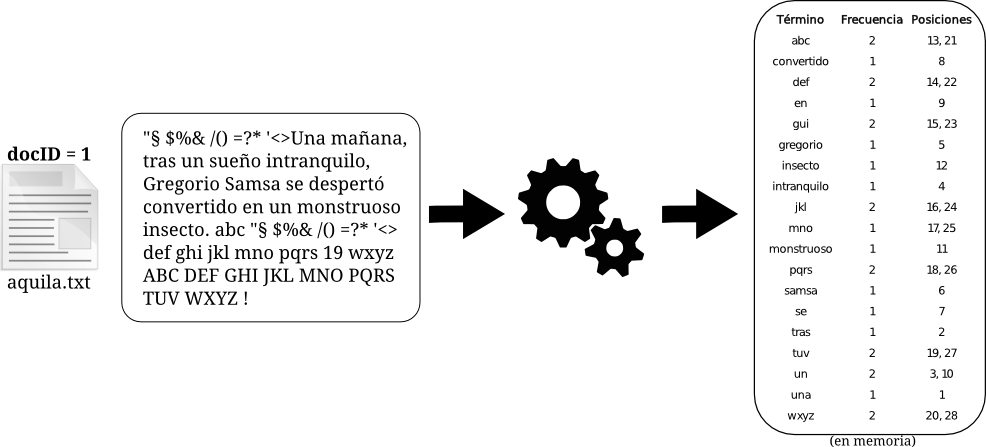
\includegraphics[scale=0.9]{./Images/parseoYMem.png}
\caption{Un archivo procesado y cargados sus términos en memoria}
\label{fig:parseoymem}
\end{figure}

Como mencionamos en la Sección \ref{sec:parser} cada término es una palabra o cifra numérica. El programa crea listados en memoria principal con la siguiente información: para un término $T_i$ se almacena que aparece en el documento con docID $D_1$ en las posiciones $p_1, p_2, p_3 \ldots p_m$, y listados equivalentes para los demás documentos. La estructura de estos listados es:

\[
\left\lbrace T_i ;
    \left( D_1 , 
        \left\langle
            p_1, p_2, p_3 \ldots p_m 
        \right\rangle  
    \right)
    ;
    \left( D_2 , 
        \left\langle
            p_1, \ldots p_f
        \right\rangle  
    \right) 
    ;
    \ldots
    ;
    \left( D_j , 
        \left\langle
            \dots
        \right\rangle  
    \right) 
\right\rbrace 
\]

Este procedimiento (generar términos y llevarlos a memorias principal) se hace constantemente hasta que ocurra uno de los siguientes hechos:

\begin{enumerate}
\item Se terminen de procesar todos los documentos
\item Se ocupe toda la memoria dedicada para el programa (se requerirán 512 MB de RAM dedicados, es decir, una PC con al menos 1 GB en total). En tal caso se crearán archivos temporales, se vaciará la memoria y se vuelve al paso 1.
\end{enumerate}


\subsection{Creación de archivos temporales}

La primera vez que ocurra uno de estos dos momentos se creará un directorio temporal <<vainillatemp/>> que irá guardando archivos temporales con la información tal cual aparece en memoria. Sucesivas bajadas de memoria a disco, generarán archivos temporales de nombre incremental.

\begin{figure}[!h]
\centering
    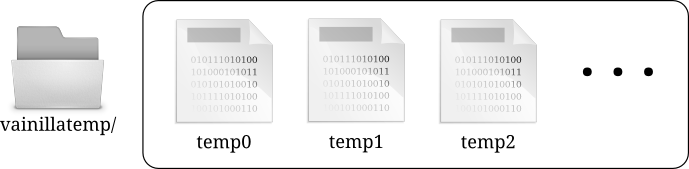
\includegraphics[scale=0.9]{./Images/tempDirEstr.png}
\caption{Un directorio temporal con archivos temporales}
\label{fig:tempdir}
\end{figure}


Cada archivo temporal contiene información suficiente para armar un índice por si mismo, ya que almacena para los documentos procesados, los términos, docIDs, frecuencias relativas y lista de posiciones como se muestra en la Figura \ref{fig:tempfile}.


\begin{figure}[!h]
\centering
    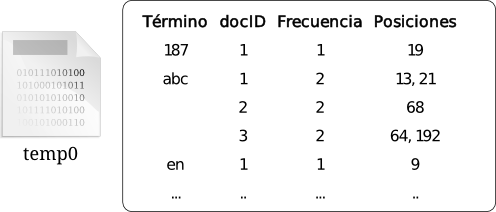
\includegraphics[scale=0.9]{./Images/tempFileEstr.png}
\caption{Un directorio temporal con archivos temporales}
\label{fig:tempfile}
\end{figure}


%\begin{figure}[here]
%\includegraphics[width=0.9\textwidth]{images/JobInformationDialog.jpg}
%\caption{A prototype of the Job Information dialog}
%\label{fig:jobInformationDialog}
%\end{figure}